\section{Relations}

\begin{definition}[Relation]
    A \textbf{relation} is a set of points in the plane.
\end{definition}

\begin{definition}[The Fundamental Graphing Principle]
    Supposing there exists a relation $R$. Plotting the points of the set $R$ in the plane, produces the \textbf{graph} of $R$
\end{definition}

\begin{definition}[The Fundamental Graphing Principle]
    The graph of an equation is the set of points which satisfices the equation that describes the relation. That is, a point $(x,y)$ is on the graph of the equation if and only if $x$ and $y$ satisfy the equation.
\end{definition}

\begin{definition}[Intercepts]
    The places where a graph crosses or touches the axes are called \textbf{intercepts}, intercepts come in two distinct varieties:
    \begin{itemize}
        \item A point on a graph which is also on the \textit{x-axis} is called an \textbf{x-intercept} of the graph
        \item A point on a graph which is also on the \textit{y-axis} is called an \textbf{y-intercept} of the graph
    \end{itemize}
\end{definition}

\begin{definition}[Finding the Intercepts of the Graph of an Equation]
    Given an equation involving $x$ and $y$, we find the intercepts of the graph as follows:
    \begin{itemize}
        \item \textit{x-intercepts} have the form $(x,0)$; set $y=0$ in the equation and solve for $x$
        \item \textit{y-intercepts} have the form $(0,y)$; set $x=0$ in the equation and solve for $y$
    \end{itemize}
\end{definition}

\begin{definition}[Testing the Graph of an Equation for Symmetry]
    To test the graph of an equation for Symmetry
    \begin{itemize}
        \item about the \textit{y-axis} - substitute $(-x, y)$ into the equation and simplify. If the result is equivalent to the original equation, the graph is symmetric about the \textit{y-axis}.
        \item about the \textit{x-axis} - substitute $(x, -y)$ into the equation and simplify. If the result is equivalent to the original equation, the graph is symmetric about the \textit{x-axis}.
        \item about the \textit{origin} - substitute $(-x, -y)$ into the equation and simplify. If the result is equivalent to the original equation, the graph is symmetric about the \textit{origin}.
    \end{itemize}
\end{definition}
\newpage

\subsection{Problems}
\begin{enumerate}
    \item [1.] \leavevmode
          \begin{center}
              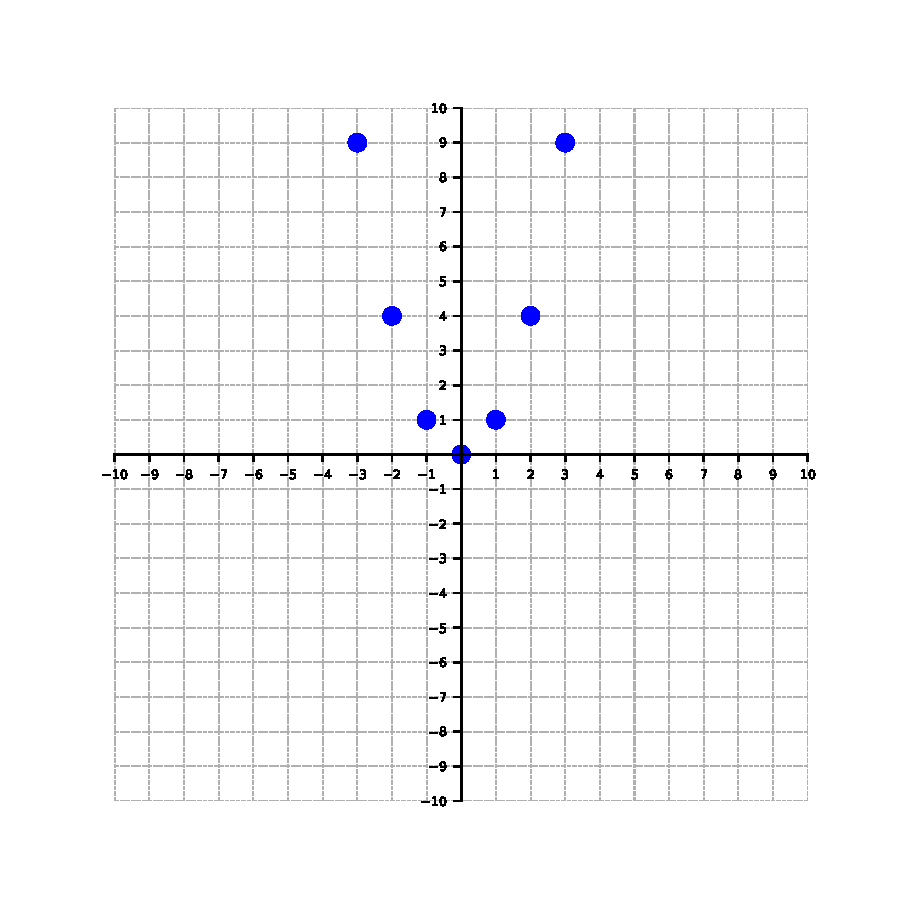
\includegraphics[width=0.5\textwidth]{figures/01_Relations_and_Functions/02_Relations/exercise_1.pdf}
          \end{center}
    \item [3.] \leavevmode
          \begin{center}
              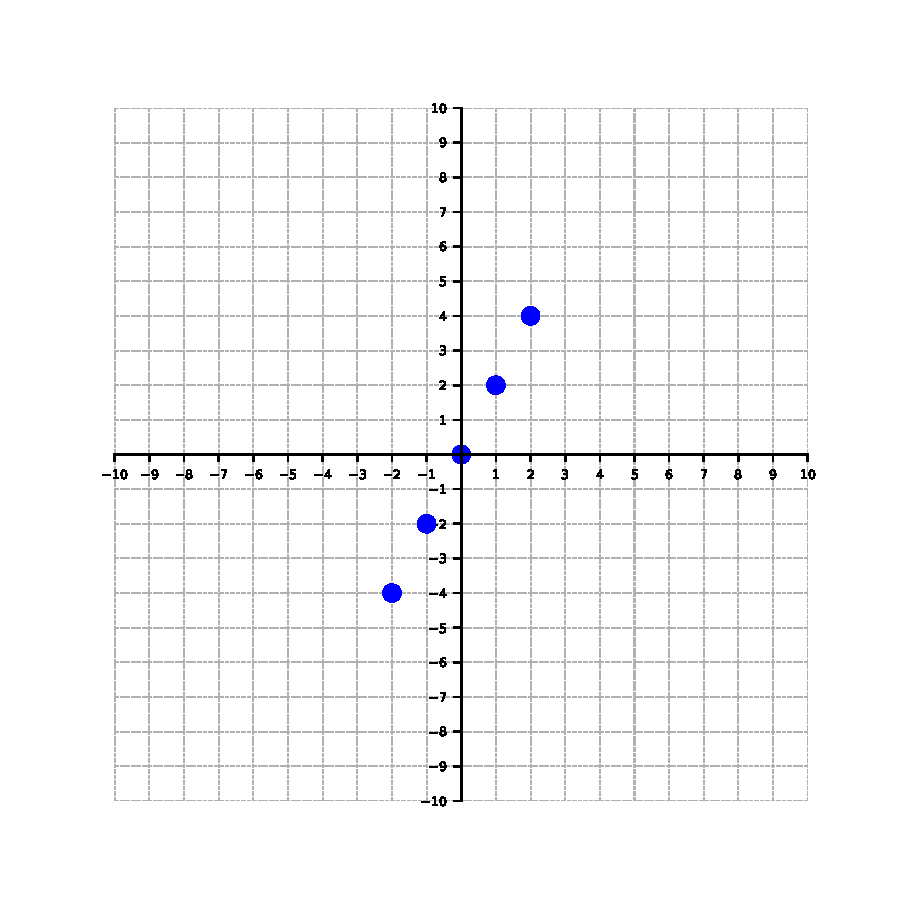
\includegraphics[width=0.5\textwidth]{figures/01_Relations_and_Functions/02_Relations/exercise_3.pdf}
          \end{center}
    \item [9.] \leavevmode
          \begin{center}
              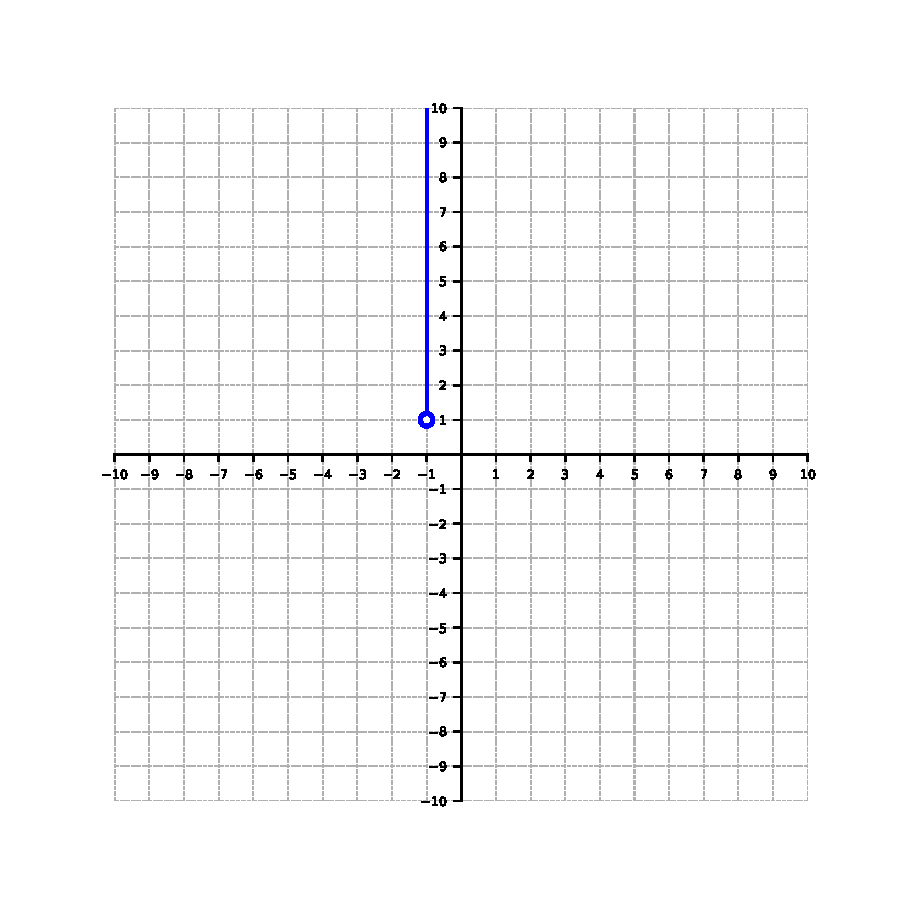
\includegraphics[width=0.5\textwidth]{figures/01_Relations_and_Functions/02_Relations/exercise_9.pdf}
          \end{center}
    \item [21.]
          \[
              \{(-4,-1),(-2,1),(0,3),(1,4)\} = \{(m, m+3) \mid m\in \{-4,-2,0,1\}\}
          \]
    \item [23.]
          \[
              \{(2, y) \mid y > -3\}
          \]
    \item [28.]
          \[
              \{(x,y) \mid -3 < x \leq 2\}
          \]
    \item [31.] \leavevmode
          \begin{center}
              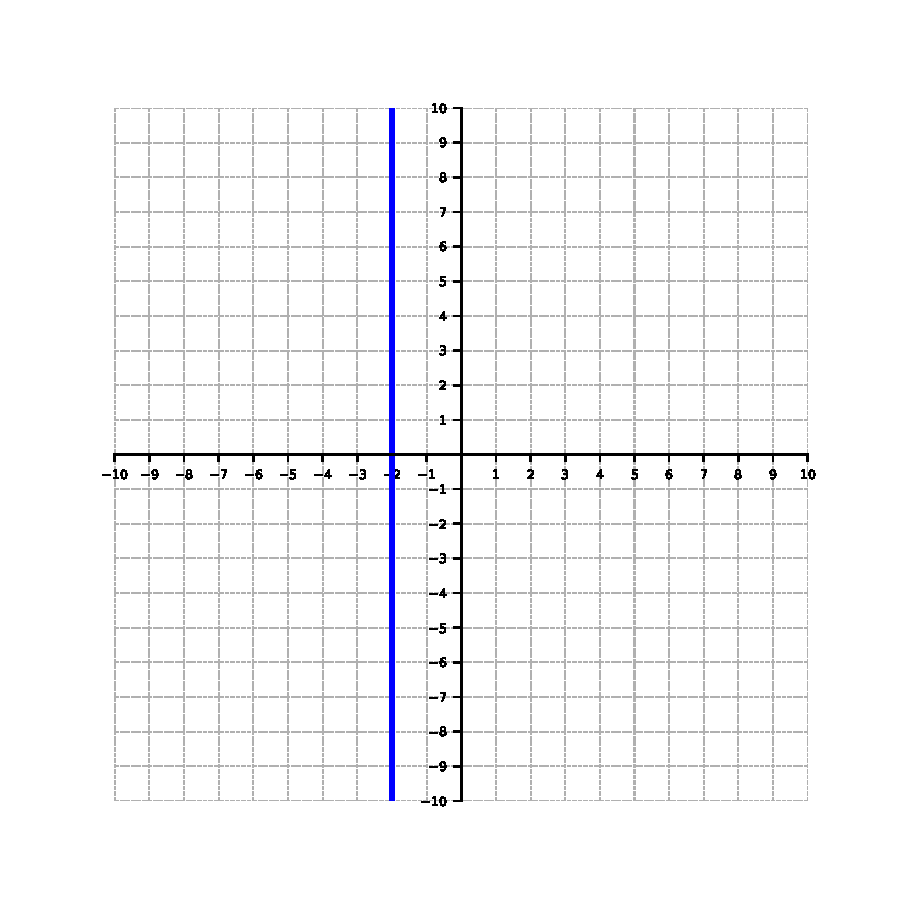
\includegraphics[width=0.5\textwidth]{figures/01_Relations_and_Functions/02_Relations/exercise_31.pdf}
          \end{center}
    \item [37.] We can start by plotting all the points for which y = 0, that is all the odd integers, then we just copy those points and translate them into the even integers on y. Will look like a grid pattern.
          Points in the relation: $(1,0), (3,2)$, Points not in the relation $(1,1),(2,2)$
    \item [39.] Practically the it is the graph of the equation $y = 2^x$
    \item [41.]
          \begin{itemize}
              \item \textit{x-intercept} doesn't exists, \textit{y-intercept} at $0$
              \item \leavevmode
                    \begin{center}
                        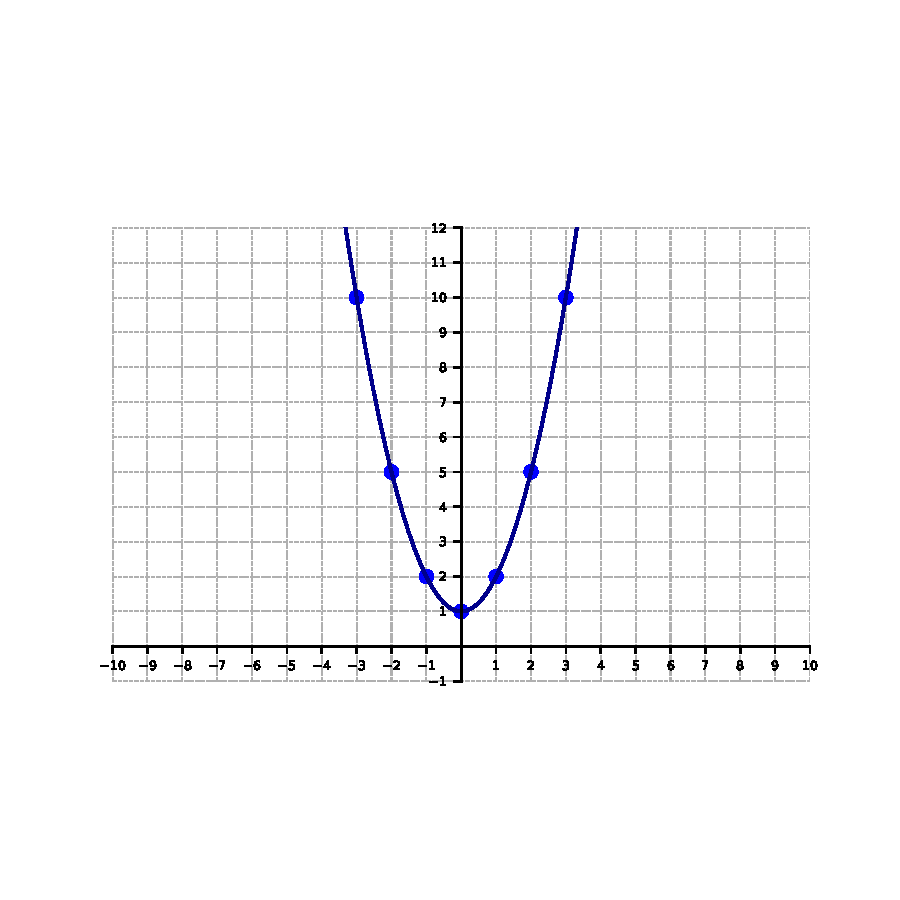
\includegraphics[width=0.5\textwidth]{figures/01_Relations_and_Functions/02_Relations/exercise_41.pdf}
                    \end{center}
              \item Graph is symmetric about the \textit{y-axis}
          \end{itemize}
    \item [47.]
          \begin{itemize}
              \item \textit{x-intercept} at $\frac{7}{3}$, \textit{y-intercept} at $-7$
              \item \leavevmode
                    \begin{center}
                        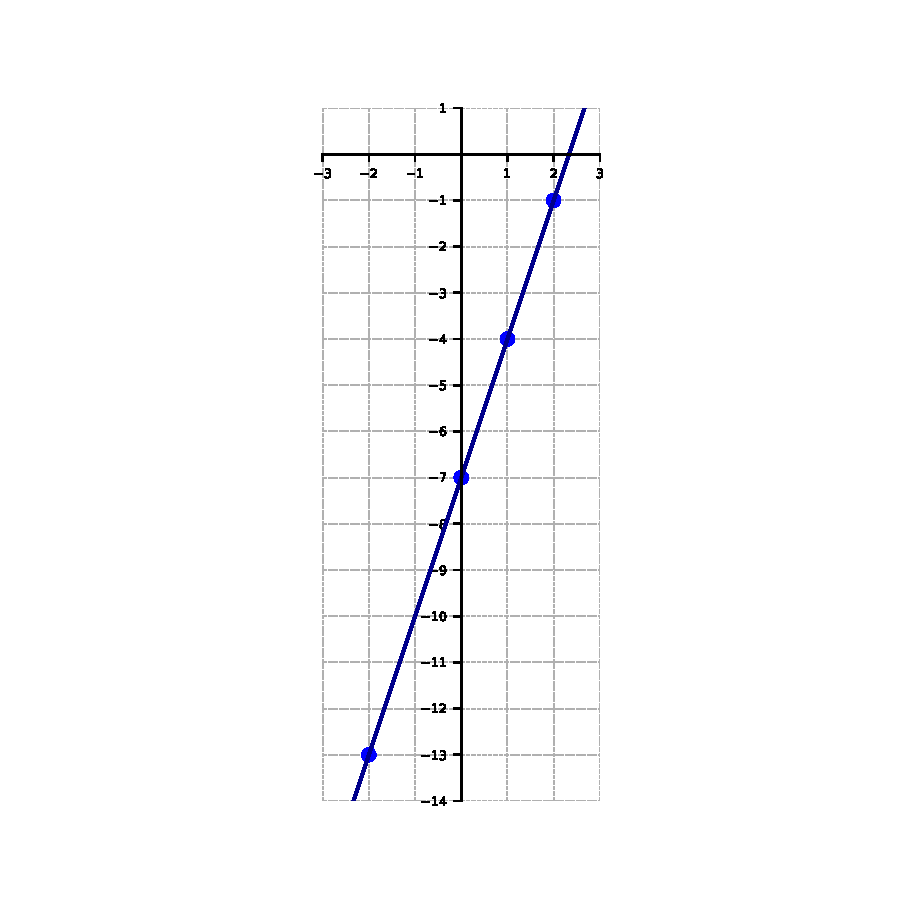
\includegraphics[width=0.5\textwidth]{figures/01_Relations_and_Functions/02_Relations/exercise_47.pdf}
                    \end{center}
              \item Graph is not symmetric, example using $-x$ we see that $y = 3x - 7 \neq -3x-7$
          \end{itemize}
    \item [53.] Multiple values of x can be multiple values of y and viceversa
\end{enumerate}